\appendix
% \renewcommand{\thesection}{\Alph{section}} % Cambia la numeración de secciones a letras
\renewcommand{\thesection}{} % Cambia la numeración de secciones a letras
% \renewcommand{\thesubsection}{\thesection.\arabic{subsection}} % Cambia la numeración de subsecciones
\renewcommand{\thesubsection}{\Alph{subsection}} % Cambia la numeración de subsecciones
% ------
\section{Appendix}
\label{sec:appendix}
% \addcontentsline{toc}{section}{Appendix} % Añadir al índice
% ------

\subsection{Second quantization} % (fold)
\label{sec:Second quantization}

The occupation-number (ON) operators are defined for the sets
of creation and annihilation operators, $\left\{ a^{\dagger} \right\}$, 
$\left\{ a \right\}$, as
\begin{equation}
    n_p = a_p^{\dagger} a_p
    .
\end{equation}

For a given ON vector $\Ket{k}$, the occupation number $k_p$ is obtained by
counting the number of electrons in spin orbital $p$
\begin{equation}
    n_p \Ket{k} =
    a_p^{\dagger} a_p \Ket{k} =
    k_p \Ket{k}
    .
\end{equation}

The ON operators are Hermitian 
\begin{equation}
    n_p^{\dagger} =
    \left( a_p^{\dagger} a_p \right)^{\dagger} =
    a_p^{\dagger} a_p =
    n_p
    ,
\end{equation}
commute among themselves 
\begin{equation}
    n_p n_q \Ket{k} =
    k_p k_q \Ket{k} =
    k_q k_p \Ket{k} =
    n_q n_p \Ket{k}
    ,
\end{equation}
and,
since in the spin-orbital basis the ON operators are projection operators,
they are idempotent, 
\begin{equation}
    n_p^2 =
    n_p n_p =
    a_p^{\dagger} a_p a_p^{\dagger} a_p =
    a_p^{\dagger} \left( 1 - a_p^{\dagger} a_p \right) a_p =
    a_p^{\dagger} a_p =
    n_p
    .
\end{equation}
Therefore, its eigenvalues can only be 0 or 1.

The particle-number operator, or simply the number operator, is the Hermitian
operator resulting from adding together all ON operators in the Fock space 
\begin{equation}
    \hat{N} =
    \sum_{p=1}^{m} a_p^{\dagger} a_p
    ,
\end{equation}
which returns the number of electrons in an ON vector 
\begin{equation}
    \hat{N} \Ket{k} =
    \sum_{p=1}^{m} k_p \Ket{k} =
    n \Ket{k}
    .
\end{equation}

Also, the $\delta_{pq}$ operator is defined as
\begin{equation}
    \delta_{pq} = a_p a_q^{\dagger} + a_q^{\dagger} a_p
    ,
\end{equation} 
which is null if $p \not= q$.

% subsubsection Second quantization (end)

\clearpage

% ---------
\subsection{Minkowski distances}
\label{sec:appendix-minkowski}
% ---------

\begin{figure}[h!]
    \centering
    % 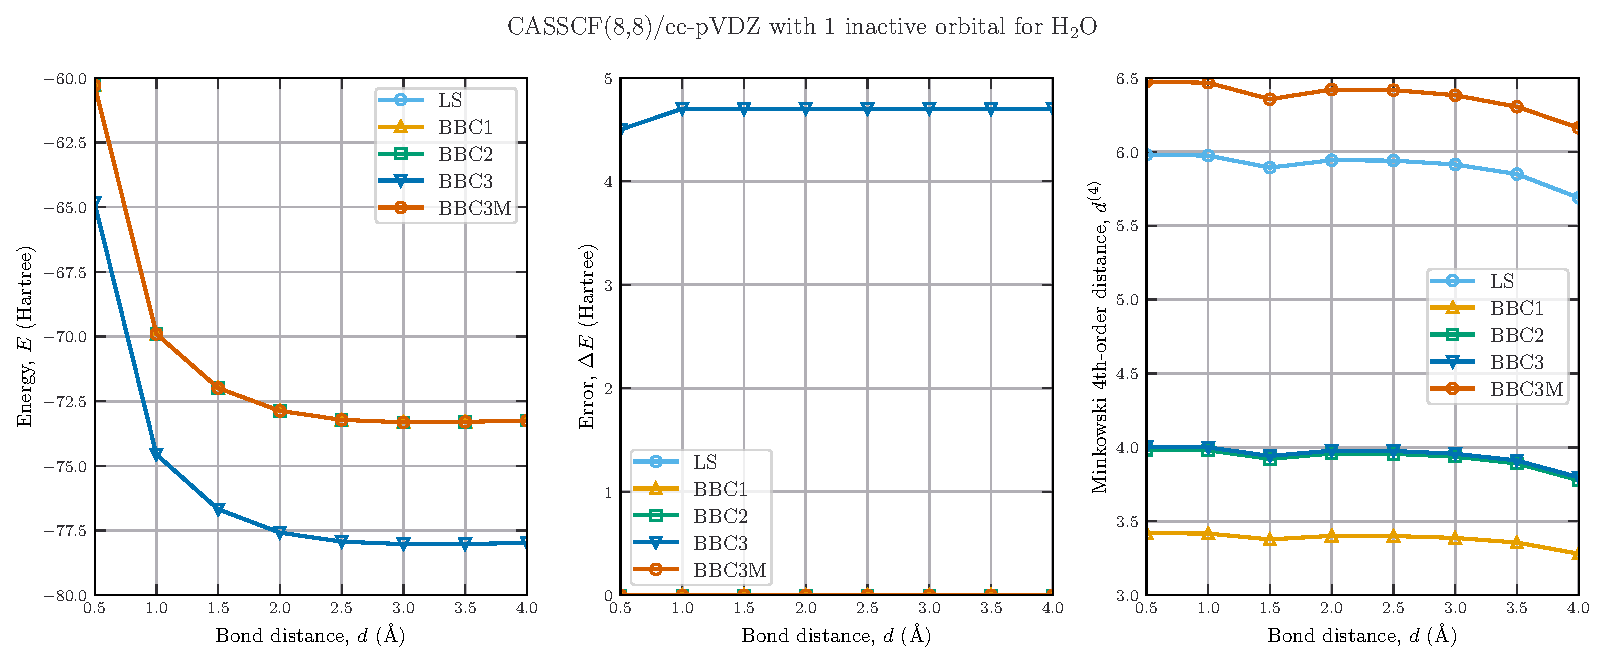
\includegraphics[width=1.0\textwidth]{MCSCF-ccpVDZ.pdf}
    \subimport{figures/}{MCSCF-ccpVDZ-minkowski.pgf}
    \caption{Minkowski distances of order $p=1,2,3,4$ for the LS, BBC1, BBC2,
    BBC3 and BBC3M approximations.}
    \label{fig:minkowski-plot}
\end{figure}

% ---------
\clearpage
\subsection{Dalton input files}
\label{sec:appendix-dalton}
% ---------
\lstinputlisting[
    language=bash,
    % firstline=2,
    % lastline=12,
    label={lst:CASSCF-input},
    caption={Dalton input file for the CASSCF(8,8) with 1 inactive orbital
    calculations for \ch{H2O}.}
]{data/DALTON.INP}

\lstinputlisting[
    language=bash,
    % firstline=2,
    % lastline=12,
    % label={lst:CASSCF-input},
    caption={Dalton \inline{.mol} input file for the \ch{H2O} molecule with 
    $d_{\ch{H-O}} = 0.5$ \AA.}
]{data/H2O-1.mol}
